\section{Introducción} \label{introduccion}
\AddToShipoutPictureBG*{
\includegraphics[width=\paperwidth,height=\paperheight]{Imagenes/Fondo Capitulo 1.pdf}}
\thispagestyle{plain}

\vspace{0.5cm}

\Large\scshape
\begin{center}
    {\Medium Configuración de la plataforma experimental y los bloques que la componen}
\end{center}
\normalfont
%\normalsize\vspace{2cm}

\divider

Previo a comenzar con el diseño de la placa de circuito impreso, debemos introducir la plataforma que se tiene que plasmar en esta PCB, explicando brevemente su funcionamiento y los bloques principales y auxiliares que la componen. Se puede apreciar un diagrama de esta plataforma, separada en sus distintos bloques funcionales en la figura \ref{fig:plataforma}.\\

\begin{figure}[h]
    \centering
    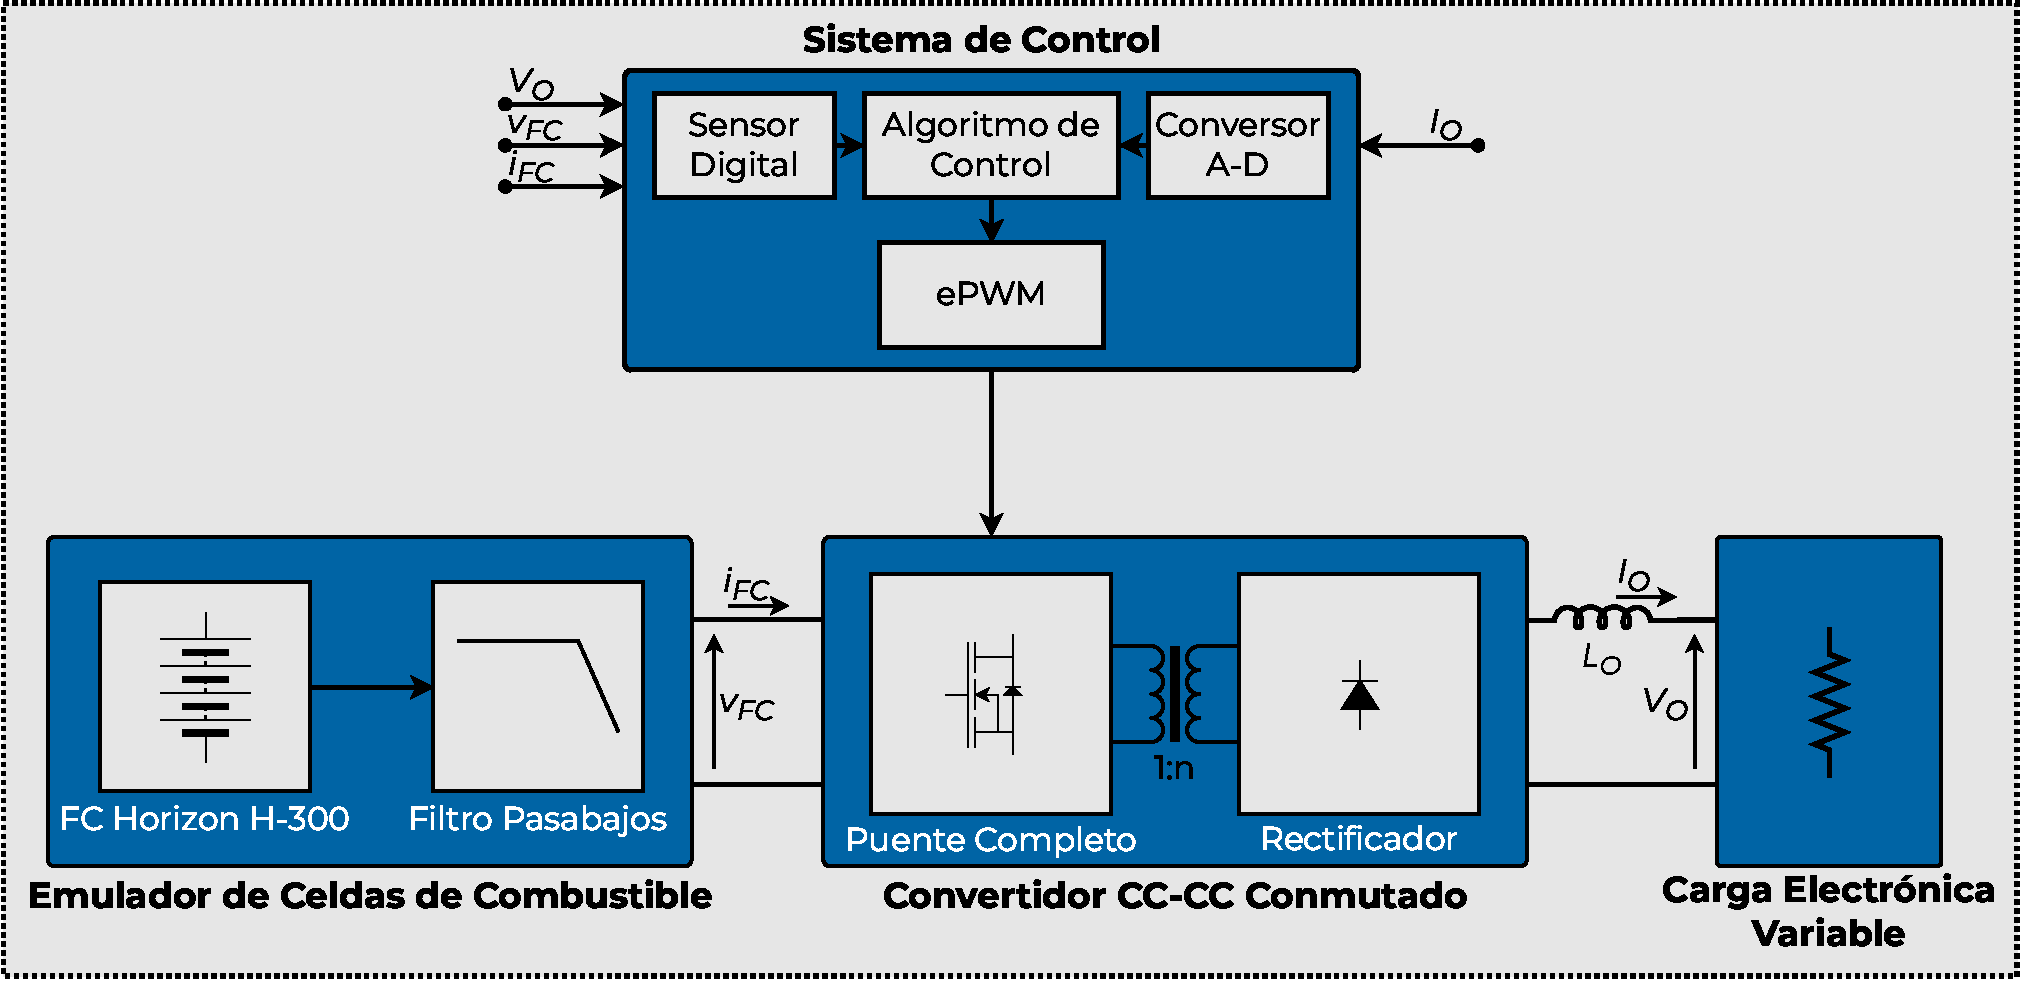
\includegraphics[scale=0.4]{Imagenes/Plataforma Experimental.pdf}
    \caption{Diagrama de la plataforma experimental de evaluación de celdas de combustible.}
    \label{fig:plataforma}
\end{figure}

Esta plataforma, como indica su nombre, tiene como objetivo la evaluación empírica de sistemas híbridos, que son sistemas de generación de energía que combinan múltiples módulos de generación y almacenamiento de energía, generalmente renovables, que luego son todos conectados a un bus de potencia, generalmente de corriente continua (CC).\\

Particularmente, este sistema evalúa el rendimiento de un módulo de generación a partir de pilas de combustible, con una tensión de pila en la entrada $v_{FC}$ variable entre \SI[]{30}[]{\volt} y \SI[]{65}[]{\volt}, y una tensión de salida común fija de \SI[]{75}[]{\volt}. Para realizar esta adaptación de niveles de tensión, se utilizó un convertidor CC-CC conmutado y aislado de tipo puente completo, que es controlado mediante el sistema de control basado en un controlador digital de señales (DSC, del inglés \textit{Digital Signal Controller}).\\

Los circuitos de estos bloques y el resto de bloques auxiliares de la figura \ref{fig:plataforma} se van a tratar uno por uno a lo largo del desarrollo de este informe, detallando su diagramas circuitales y como estos se implementaron en la plaqueta.\\